This paper presented an updated version of [REMOVED FOR BLIND REVIEW], a method for achieving a complex media annotation by running a process workflow composed of simple annotation microtasks in a cascading arrangement. Some relevant improvements were made to both the method and the framework used to support its activities.

The experiment showed that the improvements made in the method were successfully implemented, successfully generating the expected result. The contributions were obtained from a commercial crowdsourcing environment, but with a differentiated approach in which only the resources related to the workers and none of the platform resources were used. This approach ensured that both the data set used and the data collected in the contributions were stored only in our database, not the crowdsourcing platform.

It was also observed that the concept of supervised aggregation introduced in this version obtained positive results. This aggregation approach has proven to be interesting for improving the results of annotation tasks that receive open answers that need to be adjusted manually. A direct conclusion is that this approach can also be used to insert a human verification step at the end of certain aggregation activities.

The diagrams introduced considerably facilitated the creation of the workflow from the production process to the case study. In addition, a specification of the dataflow in the interfaces between the components, facilitating the planning of the distribution of the works and the information that is necessary.

The basic annotation tools distributed with the framework can be easily adapted to work with the commercial crowdsourcing platform as well as to meet the requirements of the tasks required for the experiment.

As can be seen in Figure \ref{workers}, the workers who contributed to the experiment are scattered all over the world. This ensured a heterogeneous crowd, which contributed to the operation of aggregation methods based on the wisdom theory of the crowds.
\begin{figure}[h]
	\centerline{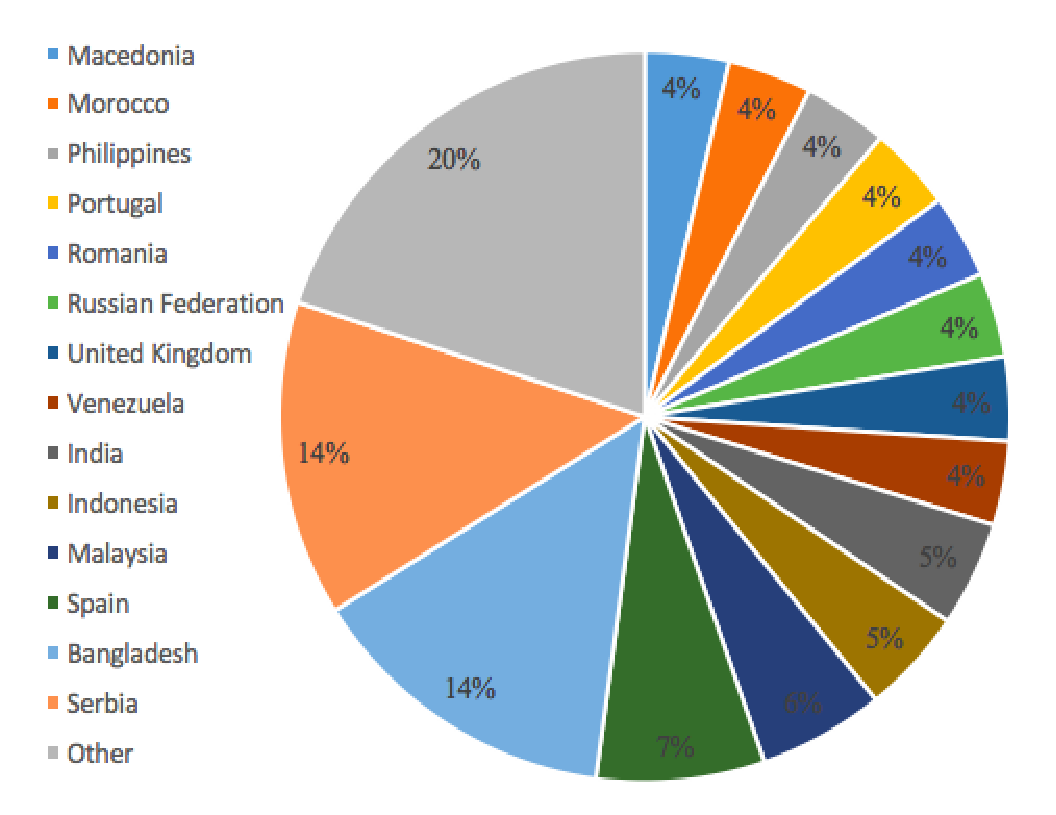
\includegraphics[scale=0.3] {figure/workers_2}}
	\caption{Workers distribution through the world.}
	\label{workers}
\end{figure}

The video enrichment process has been able to produce an interactive multimedia presentation from a simple raw video through a crowdsourcing approach. This leads to the conclusion that the updated method presented is appropriate to guide this type of project that aims to generate complex media annotations.

\subsection{Issues}
Some issues were detected in relation to the collection process. About 20\% of the contributions cannot be used because they did not meet the desired specifications or because they had invalid or malicious content. This showed that it is necessary to insert in the annotation tools some resources that induce workers to provide valid contributions. It also alerted us to the importance of giving workers clearer instructions on how to properly perform tasks.

In fact, it drew attention to the need to define criteria for the evaluation of instructions given to workers. Also came the discussion about the need for a research on whether textual instructions are really sufficient to perform any simple annotation microtasking.

\subsection{Crowds Comparison Experiment}
Another relevant discussion resulting from the observations of the results concerns the extent to which the composition of the crowd can influence the outcome.

To understand the best is not revealed, it is not a presentation method, the experiment conducted will be replicated in different scenarios:
\begin{itemize}
\item Increasing the salary of workers;
\item Choosing different contracted groups;
\item Choosing only the best workers;
\item Using a closed group with volunteers;
\item Using a group familiar with the subject treated in the video;
\item Using a group of natives in the English language.
\end{itemize}


\subsection{Next Steps}

This work is constantly improving on three different fronts: improvement of the method, improvement of the framework scenarios and application differences.

Regarding the method, the next steps include the formalization of the aggregation process, defining specific flows for automatic, supervised and manual models.

New annotation tools are being designed for the structure, which can be adapted for more tasks. In addition, a wizard is being designed to guide the creation of complex media annotation projects based on the method presented.

Some experiments are being prepared to be carried out, some of which seem especially promising:
\begin{itemize}
\item Multisensorial video annotation for mulsemedia applications.
\item Gesture segmentation in signal language video datasets.
\item Semantic approximation of idiomatic expressions in automatic translations.
\item Crowdsourcing  creation of learning object.
\end{itemize}
